\chapter{Kết quả nghiên cứu}

\section{Phương pháp tiếp cận}

Lưu ý chương này có tỉ lệ rất lớn trong điểm số của luận văn, nên sinh viên cần hết sức lưu ý việc trình bày nội dung cũng như phân tích các kết quả.

Nội dung của mục này là miêu tả về phương pháp sinh viên đã sử dụng để có các kết quả trong báo cáo.
Nếu sinh viên sử dụng phương pháp mô phỏng bằng phần mềm, thì trong mục này cần có các thông tin sau:
\begin{itemize}
\item Lưu đồ giải thuật,
\item Giải thích các khối trong lưu đồ giải thuật,
\item Các thông số điều kiện đầu vào của mô phỏng.
\end{itemize}

Nếu sinh viên thiết kế phần cứng, thì trong mục này cần có các thông tin sau:
\begin{itemize}
\item Sơ đồ khối hệ thống,
\item Giải thích các khối trong sơ đồ,
\item Sơ đồ mạch của các khối với đầy đủ thông tin về thông số linh kiện (mã số và giá trị).
\end{itemize}

Nếu sinh viên đo đạc thực nghiệm, thì trong mục này cần có các thông tin sau:
\begin{itemize}
\item Sơ đồ khối hệ thống thí nghiệm,
\item Giải thích các khối trong sơ đồ,
\item Mô tả các bước thực hiện thí nghiệm và các điều kiện khi thực hiện (thông số máy phát, máy thu, và điều kiện thí nghiệm như khoảng cách, công suất v.v).
\end{itemize}

\begin{exam}
	Sinh viên thiết kế một hệ thống phần cứng để giao tiếp với các cảm biến, có phần mềm cho vi điều khiển, và có thí nghiệm đo đạc kết quả.
	Mục này chia thành các đề mục nhỏ để mô tả riêng cho các nội dung tương ứng như sau:
	\begin{itemize}
	\item Hệ thống cảm biến
	\item Giải thuật điều khiển và thu thập dữ liệu
	\item Điều kiện thí nghiệm
	\end{itemize}
\end{exam}

Trong trường hợp sinh viên tự chứng minh được một công thức mới, hoặc tự đề xuất được một giải thuật mới chưa trình bày trong Chương \ref{sec:chuong-2}, quá trình chứng minh hoặc giải thuật mới sẽ được trình bày chi tiết trong mục này.

Việc vẽ sơ đồ khối và lưu đồ giải thuật có thể được thực hiện bằng thư viện ``tikzpicture'' đã khai báo sẵn trong mẫu báo cáo này.
Một ví dụ về giải thuật cho một giao thức điều khiển lỗi và điều khiển luồng trong môn học Truyền số liệu và Mạng thể hiện trong Hình \ref{fig:go-back-n}.
Một ví dụ khác về sơ đồ khối thí nghiệm truyền tín hiệu bằng hệ thống \ac{vlc} thể hiện trong Hình \ref{fig:so-do-thi-nghiem}.
Sinh viên có thể dùng các chương trình khác để tạo sơ đồ khối nếu muốn.

	\begin{figure}[ht]
		\centering
		\begin{tikzpicture}[node distance=2.4cm] % hiệu chỉnh khoảng cách giữa các node
		\small
		\node (io) [startstop] {Begin}; % khai bao nhãn node - loại node - tên node
		\node (buf1) [decision, below of=io] {Buffer free};
		\node (sendsn) [process, below of=buf1] {Send $SN, SN=SN+1$, timer off};
		\node (buf2) [decision, below of=sendsn] {Buffer full};
		\node (timer) [process, below of=buf2] {timer on};
		\node (ack) [decision, right of=timer, xshift=1.5cm] {ACK $RN$};
		\node (clearsn) [process, below of=ack] {Clear $SN<RN$};
		\node (nak) [decision, right of=ack, xshift=1.5cm] {NAK};
		\node (timer-out) [decision, above of=nak] {timer out};
		\node (re) [io, right of=nak, xshift=1.5cm] {Re-transmision};
		\draw [arrow] (io) -- node[anchor=south] {} (buf1); % vẽ liên kết giữa các node
		\draw [arrow] (buf1) -- node[anchor=east] {Y} (sendsn);
		\draw [arrow] (buf1) -| node[anchor=west] {N} (ack);
		\draw [arrow] (sendsn) -- node[anchor=east] {} (buf2);
		\draw [arrow] (buf2) -- node[anchor=east] {Y} (timer);
		\draw [arrow] (buf2) -| node[anchor=west] {N} (ack);
		\draw [arrow] (timer) -- node[anchor=east] {} (ack);
		\draw [arrow] (ack) -- node[anchor=east] {Y} (clearsn);
		\draw [arrow] (ack) -- node[anchor=south] {N} (nak);
		\draw [arrow] (clearsn) -| node[anchor=south] {} (nak);
		\draw [arrow] (nak) -- node[anchor=south] {Y} (re);
		\draw [arrow] (nak) -- node[anchor=east] {N} (timer-out);
		\draw [arrow] (timer-out) |- node[anchor=south] {N} (io);
		\draw [arrow] (timer-out) -| node[anchor=west] {Y} (re);
		\end{tikzpicture}
		\caption{Lưu đồ giải thuật phía phát của giao thức Go back N}
		\label{fig:go-back-n}
	\end{figure}

	\begin{figure}[ht]
		\centering
		\begin{tikzpicture}[node distance=1.75cm]
					\small
			\node (mod) [process] {Modulation};
			\node (generator) [process, above of=mod] {Arbitrary waveform generator};
			\node (driver) [process, above of=generator] {Driving cricuit};
			\node (OLED) [process, above of=driver] {OLED};
			\node (PD) [process, right of=OLED, xshift=2.5cm] {Si photodiode};
			\node (Osc) [process, below of=PD] {Oscilloscope};
			\node (demod) [process, below of=Osc] {De-modulation};
			\draw [arrow] (mod) -- (generator);
			\draw [arrow] (generator) -- (driver);
			\draw [arrow] (driver) -- (OLED);
			\draw [arrow] (OLED) -- (PD);
			\draw [arrow] (PD) -- (Osc);
			\draw [arrow] (Osc) -- (demod);
		\end{tikzpicture}
%		  \end{minipage}%
		\caption{Sơ đồ thí nghiệm hệ thống \ac{vlc}}
		\label{fig:so-do-thi-nghiem}
	\end{figure}
	
\section{Kết quả và phân tích}

Trong mục này, sinh viên trình bày các kết quả mô phỏng và đo đạc dưới dạng hình vẽ và bảng số liệu.

Đối với hình vẽ, sinh viên không được copy màn hình hoặc vẽ bằng chương trình Excel.
Sinh viên cần lưu các đồ thị kết quả ở dạng file ``.fig'' của Maltab.
Sau đó, dùng lệnh ``save as'' trong cửa sổ đồ thị của Matlab để lưu hình ảnh thành dạng file ``.eps''.
Sinh viên copy file ``.eps'' vào thư mục ``Figure'' và dùng cách chèn hình ảnh như trong Chương \ref{sec:chuong-2}.
Lý do của các bước này là file ``.eps'' là hình ảnh dạng vector, nên bảo đảm không bị nhòe hoặc bể hình khi chèn vào văn bản.
Một ví dụ hình vẽ dạng này thể hiện trong Hình \ref{fig:pho-duong}.
Sinh viên có thể so sánh Hình \ref{fig:pho-duong} với Hình \ref{fig:pho-ofdm} sẽ thấy sự khác biệt trong chất lượng hình ảnh.
Hơn nữa, việc lưu đồ thị dạng ``.fig'' giúp cho việc chỉnh sửa thông tin trên đồ thị, thêm thông số và trích thông số rất nhanh và tiện lợi.

\begin{figure} [ht]
	\begin{center}
			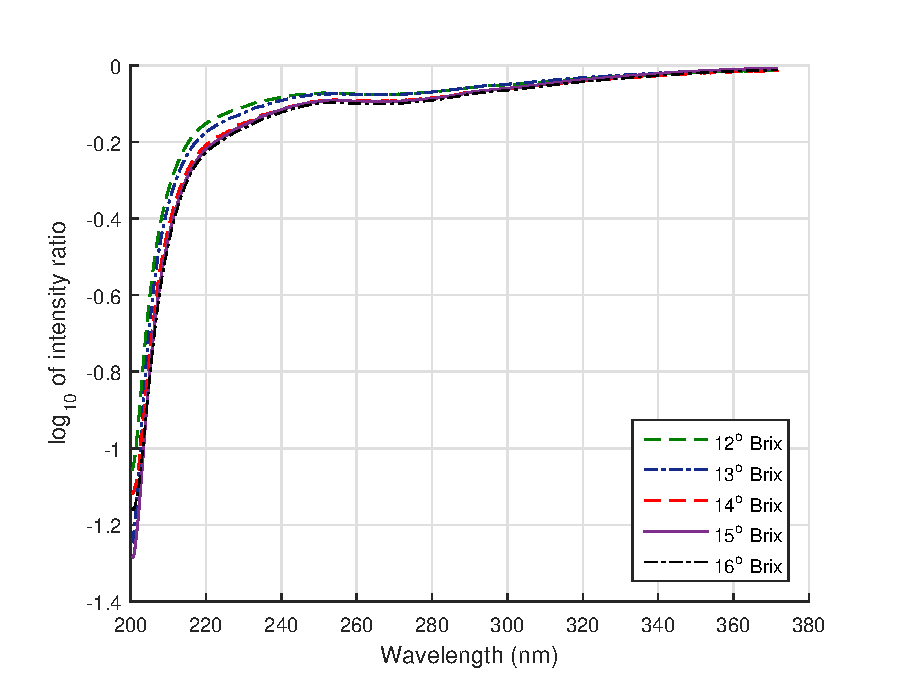
\includegraphics[width=0.75\linewidth]{thailand_conf_all_sugar.eps}
	\end{center}
	\caption{Đặc trưng nước đường từ 12 $^o$Brix đến 16 $^o$Brix} 
	\label{fig:pho-duong} 	
\end{figure} 

Khi tham khảo Hình \ref{fig:pho-duong}, sinh viên cần lưu ý các yêu cầu cơ bản của một đồ thị là phải các đủ tên và đơn vị của các trục.
Nếu có nhiều đồ thị trong một hình vẽ, sinh viên cần có bảng ``legend'' mô tả các đồ thị.
Các yêu cầu này có thể được thực hiện chính xác và nhanh chóng khi vẽ bằng Matlab.

Việc tạo bảng bằng code của Latex khá rườm rà.
Sinh viên có thể tạo bảng dễ dàng hơn bằng cách sử dụng một chương trình bảng tính khác (chẳng hạn như Excel) để tạo bảng, sau đó dùng các trang web chuyển đổi tự động sang dạng code của Latex. 
Một ví dụ của bảng dùng Latex thể hiện trong Bảng \ref{tab:cnn}.

Lưu ý hình vẽ và bảng biểu bắt buộc phải đi kèm phân tích.
Các yếu tố có thể phân tích là ý nghĩa các cực trị, nguyên nhân tăng giảm, nguyên nhân khác biệt giữa các kết quả. 

\begin{table}[ht]
	\caption{Kết quả xác suất phân loại nhãn bằng \ac{cnn}}.
	\begin{center}
	\small
		\begin{tabular}{|c|c|c|c|c|c|c|}
			\hline
			\textbf{}&\multicolumn{6}{|c|}{\textbf{Kết quả phân loại nhãn}} \\
			\cline{2-7} 
			\textbf{Nhãn} & A& B& C& D& E& F \\
			\hline
			A& 0.998& 0& 0.002& 0& 0&	0\\
			\hline
			B& 0& 0.998& 0& 0& 0&	0.002\\
			\hline
			C& 0&	0& 0.998& 0.002& 0&	0\\
			\hline
			D& 0&	0& 0.003& 0.996& 0.001& 0\\
			\hline
			E& 0& 0& 0& 0.001& 0.999& 0\\
			\hline
			F& 0&	0.003& 0& 0& 0&	0.997\\
			\hline
		\end{tabular}
		\label{tab:cnn}
	\end{center}
\end{table}

\section{Kết luận chương}

Kết luận ngắn chương 3. 
Tóm tắt lại các ý phân tích và trả lời các câu hỏi nghiên cứu.